\chapter{Оптимальное размещение базовых станций широкополосной беспроводной сети связи для обслуживания заданного множества рассредоточенных объектов}\label{ch:ch2}

Построение современной инфраструктуры передачи информации для обслуживания множества объектов промышленного или гражданского назначения, рассредоточенных на некоторой территории, является актуальной задачей при создании единой систем контроля и управления указанными объектами.  Создание такой инфраструктуры позволяет обеспечить оперативный контроль и управление объектами путем передачи необходимой информации с сенсоров и датчиков объектов в соответствующий внешнее приемное устройство. Для создания подобной инфраструктуры эффективно используются сети широкополосной беспроводной связи, необходимым этапом проектирования которых является решение задачи определения мест размещения базовых станций \cite{VishnevskyBook}.

\fixme{Широкополосные сети постепенно начинают занимать свою нишу в управлении и мониторинге нефтегазовых месторождений. В работе \cite{Mehmood2016} предложен новый протокол сенсорной сети на базе IEEE 802.11 для монторинга случаев загрязнений углеводородами.}

\fixme{А работе \cite{Abbas2021} исследуются различные протоколы сенсорных сетей для монторинга над газораспределительной городской сеть. Вся газораспределительная сеть разделена на более мелкие, управляемые сегменты, каждый из которых имеет свою базовую станцию, которая может отправлять собранные данные в центральную базу данных компании.}

В настоящей работе строятся и исследуются две математические модели задач размещения базовых станций, которые применимы на этапе синтеза топологии сети в процессе комплексного проектирования мультимедийных сетей. Предлагается модель для проверки существования допустимого решения при условия выполнении технологических ограничений для предложенной на предыдущих этапах схемы расстановки станций и модель для оптимизационной задачи. Оптимизационная задача состоит в выборе множества станций из заданного набора типов станций с различными характеристиками и их расстановки на избыточном множестве возможных мест размещения. В поставленной задаче рассматривается задача обслуживания объектов, расположение которых задано их координатами на плоскости. Особенностью такой задачи в широком классе задач оптимального размещения мощностей является наличие условия на наличие информационной связи между станциями и внешним приемным устройством (шлюзом), выполнение которого гарантирует поступление всей информации с контролируемых объектов в центр управления.

В данной главе будет предложена задача оптимального размещения базовых станций, принадлежащая к широкому классу задач размещения мощностей (Resource Allocation Problem).

\fixme{В \cite{Bukhari2021} решают задачу размещения мощностей с помощью генетического алгоритма. Авторы занимаются развертыванием устройств распределенных вычислений, серверов, вблизи устройств конечных пользователей. Связующим звеном между конечным пользователем и сервером являются базовые станции.}



% Эффективная политика кэширования контента на границе сети мобильной сотовой связи может улучшить качество услуг для мобильных пользователей и уменьшить перегрузку сети на транзитном рейсе. С другой стороны, виртуализация беспроводной сети становится передовым методом решения проблемы ограниченной пропускной способности сети из-за экспоненциального роста трафика мобильных данных. Кроме того, виртуализация беспроводной сети может принести огромные преимущества, такие как сокращение капитальных затрат (CAPEX) и эксплуатационных расходов (OPEX), а также повышение пропускной способности сети. В этом отношении одним из ключевых требований для признания преимуществ вышеупомянутых двух технологий является наличие применимой структуры распределения ресурсов, которая позволяет развертывать схемы кэширования контента в виртуализированной беспроводной сети. В этом исследовании мы исследуем новую проблему совместного распределения радиоресурсов и кэширования контента, чтобы эффективно использовать блоки радиоресурсов, мощность передачи и доступную кэш-память на базовых станциях (BS). Цель сформулированной проблемы, представленной в этой статье, направлена ​​на минимизацию задержек, с которыми сталкиваются конечные мобильные пользователи операторов мобильных виртуальных сетей (MVNO). Мы показываем, что сформулированная задача является невыпуклой смешанной целочисленной нелинейной задачей (MINLP), которая NP-трудна и просто неразрешима. Поэтому мы применяем алгоритм блочной минимизации верхней границы (BSUM) для решения сформулированной задачи. Численные результаты показывают, что наш метод превосходит существующие базовые схемы распределения ресурсов с приростом производительности до 19% с точки зрения сетевой задержки.}

В рамках широкого класса задач размещения мощностей в наших задачах размещения присутсвует специфика на связь между всеми узлами сети и наличие линейной траектории в случае задачи с линейной топологией.


\section{Задача при заданных местах размещения станций.}

Задано множество вершин $A= \left\{ a_i \right\}, i=\overline{0,n}$ на плоскости. Каждая вершина $a_i$ имеет координаты $\left\{ x_i, y_i \right\}$.

Множество $A$ состоит из двух подмножеств:
\begin{itemize}
    \item $A_1$ –- множество вершин, которое соответствует объектам, с которых необходимо собирать информацию. Каждой вершине $a_i$ приписана величина $v_i$ -– максимальный объем информации, снимаемой с объекта, расположенного на этой вершине. В частности, объектами могут быть любые стационарные абонентские устройства сети 802.11n. В дальнейшем будем считать, что каждая вершина из $A_1$ является объектом контроля.
    \item $A_2$ =– множество мест, где размещены базовые станции. В дальнейшем вершину из $A_2$ будем идентифицировать  не только как место размещения, но и как соответствующую станцию.
\end{itemize}

По определению:
$$
A_1 \cup A_2 = \varnothing;
$$

$$
A_1 \cap A_2 = A.
$$

Все вершины пронумерованы так,что:
$$
A_1 = \left\{a_i \right\}, i= \overline{1,n_1};
$$

$$
A_2 = \left\{ a_i  \right\}, i= \overline{n_1+1,n}.
$$

Каждой вершине из $A_2$ приписаны три параметра $s_i = \left\{ r_i, R_{ij},\vartheta_i \right\} $, где:

\begin{itemize}
    \item $r_i$ -- максимальный радиус покрытия станции. Параметр, который характеризует зону охвата территории каждой станцией;
    \item $R_{ij}$ -- максимальный радиус связи между $i$-ой и $j$-ой станциями. Параметр характеризует расстояние, на котором обеспечивается связь между станциями;
    \item $\vartheta_i$ -- максимальный объем информации в единицу времени, который может быть получен от объектов, обслуживаемых станцией.
\end{itemize}

Также задана вершина специального вида (шлюз) $s_0 = \left\{ r_0, R_0, \vartheta_0 \right\} $ с координатами $\left\{x_0, y_0 \right\}$. По условию задачи величина $\vartheta_0$ больше суммы величин $\vartheta_i$ у всех вершин множества $A_1$.

Задано условие, что со шлюзом и между собой могут быть связаны только вершины множества $A_2$.

Требуется проверить, что при заданных наборе и размещении станций вся имеющаяся информация с объектов (множество $A_1$) может быть собрана и передана системой станций (множество $A_2$) до шлюза $s_0$.

Сформулируем задачу в виде модели \fixme{ЛП}.

Составим граф $ H = \left\{A,E \right\} $ для возможного потока информации между вершинами множества $ A = A_1 \cup A_2 $. По определению, каждой вершине из $ A_2 $ соответствует свой набор параметров $\left\{ r_i  R_i, \vartheta_i \right\} $.
Матрица смежности $E = \left\{ e_{ij} \right\}$ графа $H$ строится по следующим правилам:

\begin{itemize}
    \item $e_{ij} = 1$, если расстояние между $i$-ым объектом ($a_i \in A_1$) и $j$-ым местом размещения станции ($a_j \in A_2$) не более радиуса покрытия для станции соответствующего этой вершине типа; 
    \item $e_{ij} = 1$, если расстояние между $i$-ым местом размещения ($a_i \in A_2$) и $j$-ым местом размещения  ($a_j \in A_2$), не более радиуса связи той станции, у которой радиус связи не больше радиуса связи другой станции;
    \item $e_{i0} = 1$, если расстояние от вершины $a_i \in A_2$ до шлюза не более $R_i$;
    \item $e_{ij} = 0$, во всех остальных случаях.
\end{itemize}

Введем переменные $x_{ij} \geqslant 0$. Это искомое количество информации, передаваемой в единицу времени по дуге $e_{ij}$ графа $H$.
Распишем условия для нашей задачи.
Величина суммарного потока, который выходит с объекта равен весу $\vartheta_i$:

\begin{equation}\label{eq:part2_1.1}
    \sum_{a_j \in \Gamma^+(a_i)} x_{ij} = \vartheta_i, \forall a_i, i=\overline{1, n_1},
\end{equation}
где $\Gamma^+(a_i)$ – множество вершин на графе $H$, в которые входят дуги, исходящие из вершины $a_i$. 

Сумма входящих и выходящих потоков для любой $i$-ой вершины множества $A_2$ равна нулю:

\begin{equation}\label{eq:part2_1.2}
    \sum_{a_j \in \Gamma_1^-(a_i)} x_{ij} + \sum_{a_j \in \Gamma_2^-(a_i)} x_{ji} -  \sum_{a_j \in \Gamma_2^+(a_i)} x_{ij} =0 ,\forall a_i \in A_2. 
\end{equation}

Здесь множество $\Gamma_1^-(a_i)$ – вершины множества $A_1$, из которых выходят дуги, входящие в вершину $a_i$, $\Gamma_2^-(a_i)$ – вершины множества $A_2$, из которых выходят дуги, входящие в  вершину $a_i$, $\Gamma_2^+(a_i)$ – вершины множества $A_2$, в которые входят дуги, исходящие из вершины $a_i$.

Через систему станций вся информация от объектов  должна поступить  на шлюз $s_0$:

\begin{equation}\label{eq:part2_1.3}
    \sum_{a_j \in \Gamma_2^-(a_0)} x_{j0} =  \sum_{a_i \in A_1} \vartheta_i;
\end{equation}

Объем информации, поступающей с других вершин на станцию, если она размещена на $j$-ой вершине, ограничен мощностью станции $\vartheta_j$:

\begin{equation}\label{eq:part2_1.4}
    \sum_{a_j \in \Gamma^-(a_i)} x_{ji} \leqslant \vartheta_j, \forall a_j \in A_2D.
\end{equation}

Для нахождение допустимого решения задачи \cref{eq:part2_1.1, eq:part2_1.2, eq:part2_1.3, eq:part2_1.4} (или доказательства, что допустимого решения не существует) может быть применена стандартная процедура нахождения допустимого решения задачи линейного программирования с вводом искусственных переменных в уравнения \cref{eq:part2_1.1, eq:part2_1.2, eq:part2_1.3, eq:part2_1.4} и минимизации состоящей из этих переменных линейной формы. Если значение целевой функции в результате решения задачи окажется больше нуля, то допустимого решения для данного размещения станций не существует, в противном случае полученное решение дает допустимое распределение потоков по каналам связи.

\section{Оптимизационная задача выбора набора размещаемых станций и определения мест их размещения}
Постановка задачи
Задано множество вершин $A = a_i$, $i=\overline{0,n}$ на плоскости. Каждая вершина $a_i$ имеет координаты $\left\{ x_i, y_i \right\}$.
Множество $A$ состоит из двух подмножеств: 
\begin{itemize}
    \item $A_1$ -- множество вершин, с которых необходимо собирать информацию. Каждой вершине $a_i$ приписана   величина $v_i$ -- максимальный объем информации, снимаемой с объекта, расположенного на этой вершине;
    \item $A_2$ -- множество возможных мест размещения базовых станций. 
\end{itemize}

По определению

$$
A_1 \cup A_2 = \varnothing;
$$

$$
A_1 \cap A_2 = A.
$$

Все вершины пронумерованы так, что:

$$
A_1 = \left\{a_i \right\}, i= \overline{1,n_1};
$$

$$
A_2 = \left\{ a_i  \right\}, i= \overline{n_1+1,n}.
$$


Задано множество типов базовых станций $S = s_j$, $j=\overline{1,m}$, которые необходимо разместить на множестве $A_2$.

Каждой станции приписаны четыре параметра $s_j = \left\{r_j, R_j, \vartheta_j, c_j \right\}$, где: 
\begin{itemize}
    \item $r_j$ -- максимальный радиус покрытия;
    \item $R_{ij}$ -- максимальный радиус связи между $i$-ой и $j$-ой станциями. Параметр характеризует расстояние, на котором обеспечивается связь между станциями;
    \item $\vartheta_j$ -- максимальный объем информации в единицу времени, который может быть получен от объектов, обслуживаемых данной станцией;
    \item $c_j$ -- стоиомость станции.
\end{itemize}

Также задана станция специального вида (шлюз) $s_0 = \left\{ r_0, R_0, \vartheta_0, c_0 \right\}$ с координатами $\left\{x_0, y_0 \right\}$, где $r_0 = R_0 = \vartheta_0 = c_0 = 0$


Требуется разместить станции таким образом, чтобы вся информация с объектов (вершинах множества $A_1$) могла быть собрана и передана системой станций, размещенных на выбранных в результате решения задачи вершинах множества  $A_2$, до шлюза $s_0$ и общая стоимость размещенных станций была бы минимальной.
Как и в предыдущих задачах вершины и станции будем, соответственно, идентифицировать как объекты или станции на них размещенные.
Задано условие, что информация c вершин множества $A_1$ может передаваться непосредственно только на вершины множества $A_2$, а со шлюзом и между собой могут быть связаны только вершины множества $A_2$.

\fixme{Заметим, что в отличие от предыдущих двух задач в данной задаче задано не множество станций, которые все должны быть использованы в проектируемой сети, а только типы станций. Таким образом в результате решения задачи определяется как набор станций, так и места их размещения.}
Формулировка задачи в виде модели частично целочисленного ЛП.
Вместо каждой вершины $ai$, $i= \overline{n_1+1,n}$ введем $m$ вершин с координатами вершины $a_i$, и различными параметрами, соответствующими различным типам станций. Обозначим такую группу вершин, записанных с одинаковыми координатами вместо вершины $a_i$,как $D_i$. Каждой вершине из $D_i$ поставим в соответствие набор параметров только одного типа станции из $S$, т.е. на данной вершине может стоять либо станция приписанного типа либо никакая. Обозначим расширенное множество вершин $A_2$ через $A_2D$.

Составим граф $H=\left\{AD,E\right\}$, описывающий сеть для передачи потока информации между вершинами расширенного множествa $AD=A_1 \cup A_2D$ и шлюзом.
Матрица смежности $E = e_{ij}$ графа $H$ строится по следующим правилам.

\begin{itemize}
    \item $e_{ij} = 1$, если расстояние между $i$-ой вершиной ($a_i \in A_1$) и $j$-ой вершиной ($a_j \in A_2D$) не более радиуса покрытия, приписанного этой вершине;
    \item $e_{ij} = 1$, если вершины $a_i$ и $a_j$   принадлежат разным множествам $D_i$ и $D_j$ и расстояние между ними не более радиуса связи той вершины, у которой радиус связи не больше радиуса связи другой вершины;
    \item $e_{i0} = 1$ ($a_i \in A_2D$ ) если расстояние от вершины до шлюза не более $R_i$;
    \item $e_{ij} = 0$, во всех остальных случаях.
\end{itemize}

Введем потоковые переменные $x_{ij} \geqslant 0$.

Распишем условия для нашей задачи.
Величина суммарного потока, который выходит с вершины $a_i$ равен весу $\vartheta_i$ \cref{eq:part2_1.5}

\begin{equation}\label{eq:part2_1.5}
    \sum_{a_j \in \Gamma^+(a_i)} x_{ij} = \vartheta_i, \forall a_i, i =\overline{1, n_1};
\end{equation} 
где $\Gamma^+(a_i)$ -- множество вершин на графе $H$, в которые входят дуги, исходящие из вершины $a_i$.

Сумма входящих и выходящих потоков для любой $i$-ой вершины множества $A_2D$ равна нулю \cref{eq:part2_1.6}
\begin{equation}\label{eq:part2_1.6}
    \sum_{a_j \in \Gamma_1^-(a_i)} x_{ij} + \sum_{a_j \in \Gamma_2^-(a_i)} x_{ji} -  \sum_{a_j \in \Gamma_2^+(a_i)} x_{ij} =0 ,\forall a_i \in A_2. 
\end{equation} 
Здесь множество $\Gamma_1^-(a_i)$ -- вершины множества $A_1$, из которые выходят дуги, входящие в вершину $a_i$, $\Gamma_2^-(a_i)$ -- вершины множества $A_2D$, из которых выходят дуги, входящие в  вершину $a_i$, $\Gamma_2^+(a_i)$ -- вершины множества $A_2D$, в которые входят дуги, исходящие из вершины  $a_i$.

Через систему станций вся информация от объектов  должна поступить на шлюз $s_0$ 
\begin{equation}\label{eq:part2_1.7}
    \sum_{a_j \in \Gamma_2^-(a_0)} x_{j0} = \sum_{a_i \in A_1} \vartheta_i.
\end{equation}
Здесь $\Gamma_2^-(a_0)$ –- подмножество вершин множества $A_2D$, дуги которых входят в шлюз $a_0$.

Введем булевы переменные $y_i$ для вершин $a_i$, $a_i \in A_2D$
\begin{itemize}
    \item $y_i = 1$, если станция стоит на месте $a_i$;
    \item $y_i = 0$, в противном случае.
\end{itemize}

Объем информации, поступающей от вершин множества $A_1$ на вершину $a_i \in A_2D$, ограничен мощностью станции $\vartheta_i$ \cref{eq:part2_1.8}
\begin{equation}\label{eq:part2_1.8}
    \sum_{a_j \in \Gamma^-(a_i)} x_{ji} \leqslant y_i \cdot \vartheta_i, \forall a_i \in A_2D.
\end{equation}

На множестве $D_i$ может быть размещено не более одной станции \cref{eq:part2_1.9}
\begin{equation}\label{eq:part2_1.9}
    \sum_{a_j \in D_i} y_j \leqslant 1, \forall D_i.
\end{equation}

Целевая функция

\begin{equation}\label{eq:part2_1.10}
    \sum_{a_i \in A_2D} c_i \cdot y_i \to min.
\end{equation}

Задача \cref{eq:part2_1.5, eq:part2_1.6, eq:part2_1.7, eq:part2_1.8, eq:part2_1.9, eq:part2_1.10} представляет собой частично целочисленную задачу линейного программирования с $m \cdot |A_2|$ булевыми переменными.

Численный пример решения задачи оптимизации представлен в Приложении \cref{app:milp_place_solution}.

% \section{Пример решения задачи}
% Рассмотрим пример для оптимизационной задачи выбора набора размещаемых станций и определения мест их размещения.
% Задано множество рассредоточенных объектов $A_1$, $|A_1| = 4$ и шлюз (таблица \cref{tab:part2_placement_coordinates}).

% \begin{table}
%     \centering
%     \captionsetup{justification=centering} % выравнивание подписи по-центру
%     \caption{Координаты размещения}\label{tab:part2_placement_coordinates}
%     \begin{tabular}{|l|c|c|}
%         \toprule
%         0   & (7,4) & \textbf{Координаты шлюза} \\
%         \midrule
%         1   & (1, 5)& \textbf{Координаты объектов}  \\
%         2   & (4.5, 4) & \\
%         3   & (6, 3) & \\
%         4   & (3.5, 5) & \\
%         \midrule
%         5   & (2, 4) & \textbf{Координаты размещения станций}  \\
%         6   & (5, 5) & \\
%         7   & (2, 6) & \\
%         8   & (6, 5.5) & \\
%         \bottomrule
%     \end{tabular}
% \end{table}

% Задано множество $A_2$ возможных мест расположения станций, $|A_2| = 4$. Все вершины представлены на рисунке \ref{fig:part2_coordinates}.
 
% \begin{figure}[ht]
%     \centerfloat{
%         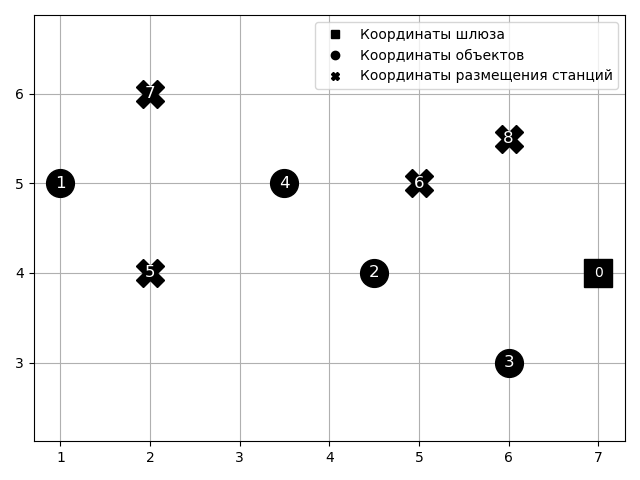
\includegraphics[scale=0.75]{part2_coordinates.png}
%     }
%     \caption{Координаты размещения}\label{fig:part2_coordinates}
% \end{figure}

% Задано ограничение по мощности для кадого объекта (таблица \ref{tab:part2_object_capacity}).

% \begin{table}
%     \centering
%     \captionsetup{justification=centering} % выравнивание подписи по-центру
%     \caption{Координаты размещения}\label{tab:part2_object_capacity}
%     \begin{tabular}{|c|cccc|}
%         \toprule
%         Объекты   & 1 & 2 & 3 & 4 \\
%         \midrule
%         Мощность  & 10 & 15 & 17 & 18 \\
%         \bottomrule
%     \end{tabular}
% \end{table}

% Задано множество типов станций (таблица \ref{tab:part2_station_types}).

% \begin{table}
%     \centering
%     \captionsetup{justification=centering} % выравнивание подписи по-центру
%     \caption{Множество типов станций}\label{tab:part2_station_types}
%     \begin{tabular}{|c|c|c|c|c|}
%         \toprule
%         Тип & Мощность, $\vartheta_j$ & Радиус покрытия, $r_j$  & Радиус связи, $R_j$ & Стоимость, $c_j$ \\
%         \toprule
%         1   & 80 & 1 & 6 & 70 \\
%         2  & 100 & 2 & 5 & 75 \\
%         3  & 100 & 2 & 5 & 75 \\
%         \bottomrule
%     \end{tabular}
% \end{table}

% Необходимо разместить станции таким образом, чтобы минимизировать их  суммарную общую стоимость.
% Построим граф сети $H$ для данного набора типов станции. Матрица смежности представлена на рисункке \cref{fig:part2_adjacency_matrix}
 
% \begin{figure}[ht]
%     \centerfloat{
%         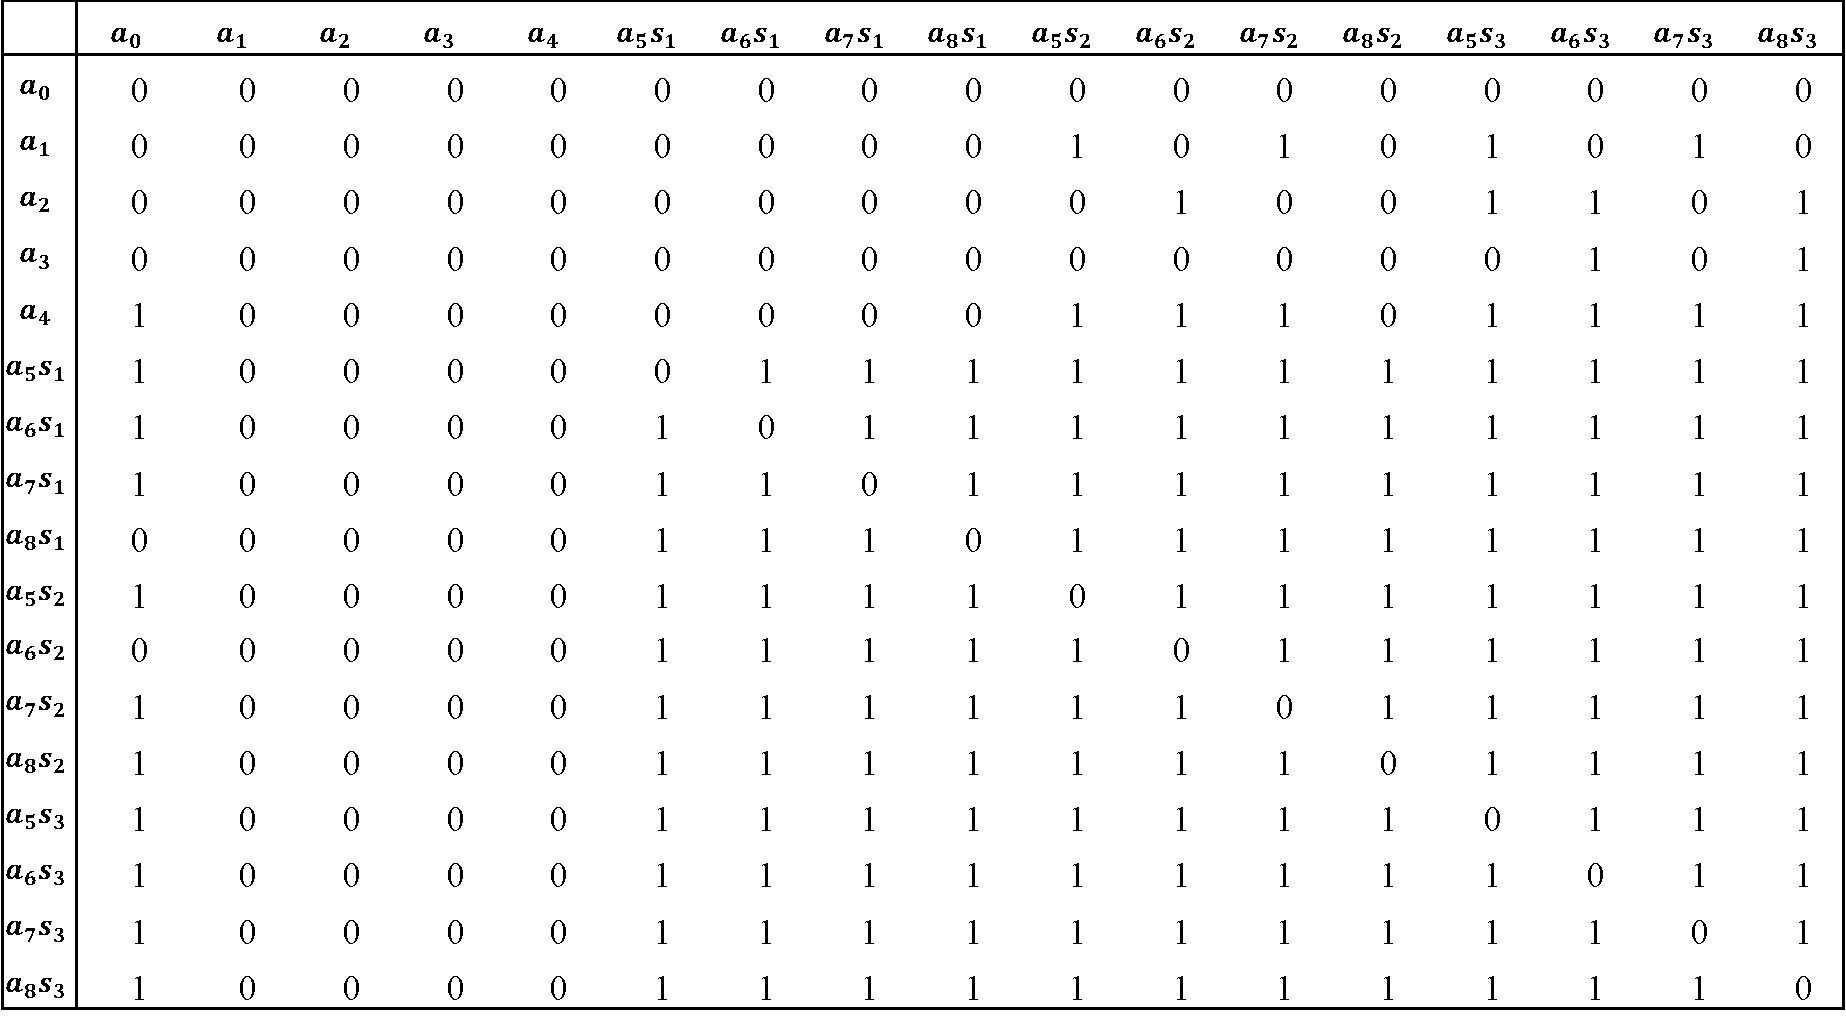
\includegraphics[scale=0.5]{part2_adjacency_matrix.pdf}
%     }
%     \caption{Координаты размещения}\label{fig:part2_adjacency_matrix}
% \end{figure}

% % \begin{table}
% %     \centering
% %     \captionsetup{justification=centering} % выравнивание подписи по-центру
% %     \caption{Матрица смежности графа $H$}\label{tab:part2_adjacency_matrix}
% %     \begin{tabular}{|c|c|c|c|c|c|c|c|c|c|c|c|c|c|c|c|c|}
% %         \toprule
% %         a_0 & a_1 & a_2 & a_3 & a_4 & a_5s_1 & a_6s_1 & a_7s_1 & a_8s_1 & a_5s_2 a_6s_2 & a_7s_2 & a_8s_2 & a_5s_3 & a_6s_3 & a_7s_3 & a_8s_3 \\
% %         \toprule
% %         1   & 80 & 1 & 6 & 70 \\
% %         2  & 100 & 2 & 5 & 75 \\
% %         3  & 100 & 2 & 5 & 75 \\
% %         \bottomrule
% %     \end{tabular}
% % \end{table}


% На основе матрицы смежности полученного графа запишем систему равенств и неравенств\cref{eq:part2_1.5, eq:part2_1.6, eq:part2_1.7, eq:part2_1.8, eq:part2_1.9, eq:part2_1.10} и решим задачу частично целочисленного ЛП.
% В ходе решения мы получили следующее размещение станции (рис. \cref{fig:part2_solution})

% \begin{figure}[ht]
%     \centerfloat{
%         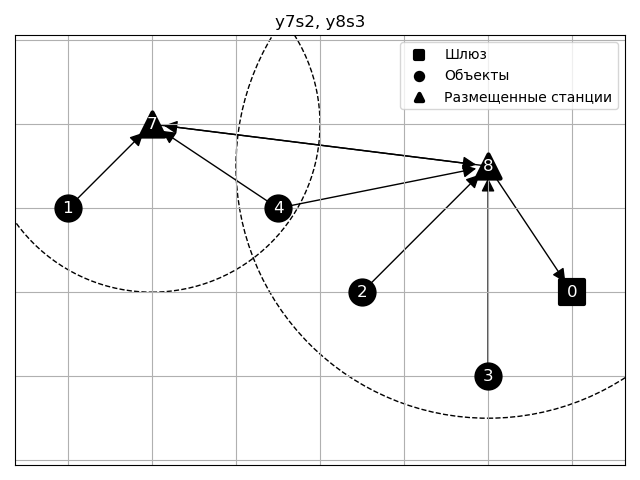
\includegraphics[scale=0.75]{part2_solution.png}
%     }
%     \caption{Координаты размещения}\label{fig:part2_solution}
% \end{figure}

% Из графика видно, что были размещены на точках 7 и 8 две станции типа 2 и 3, соответственно.
% Решением задачи является суммарная стоимость равная:
% $f=160$.





% % \section{Результаты численного эксперимента}

% Алгоритмы построения графов $H$ были запрограммированы на языке Python. Задачи, сформулированные на основании графов $H$ в виде соответствующих задач математического программирования, были решены пакетом Optimization Toolbox MATLAB.
% В таблице 4 представлены результаты времени счета задач частично целочисленного ЛП для различных случаев числа мест размещения станций и числа объектов. Для каждого случая было проведено по 10 примеров.

% \begin{table}
%     \centering
%     \captionsetup{justification=centering} % выравнивание подписи по-центру
%     \caption{Множество типов станций}\label{tab:part2_station_types}
%     \begin{tabular}{|c|c|c|}
%         \toprule
%         Количество & Количество мест  & Среднее время 
%         \tabularnewline объектов, $n_1$ & размещения станций, $n-n_1$ &  счета, сек.  \\
%         \toprule
%         4   & 3 & 12,34 \\
%         4   & 4 & 12,42 \\
%         4   & 5 & 12,31 \\
%         6   & 6 & 11,20 \\
%         8   & 7 & 11,27 \\
%         10  & 7 & 12,32 \\
%         12  & 10 & 12,51 \\
%         14  & 7 & 12,42 \\
%         17  & 8 & 12,18 \\
%         21  & 8 & 12,53 \\
%         25  & 8 & 14,22 \\
%         \bottomrule
%     \end{tabular}
% \end{table}

\section{Выводы к главе 2}
В работе рассмотрены задачи размещения базовых станций при проектировании беспроводных широкополосных сетей связи. Предложены формулировки задач в виде   моделей линейного и частично целочисленного линейного программирования как для случая проверки  наличия допустимых решений для вариантов, предложенных проектировщиками, так и для экстремальной задачи отбора множества станций из имеющегося набора типов станций и оптимального размещения станций выбранного множества на избыточном множестве возможных мест размещения. Предложены алгоритмы построения графов информационных потоков, позволившие формализовать задачи в виде соответствующих моделей математического программирования. Приведены результаты вычислительного эксперимента.


















% \section{Одиночное изображение}\label{sec:ch2/sec1}

% \begin{figure}[ht]
%     \centerfloat{
%         
\includegraphics[scale=0.27]{latex}
%     }
%     \caption{TeX.}\label{fig:latex}
% \end{figure}



% Для выравнивания изображения по-центру используется команда \verb+\centerfloat+, которая является во
% многом улучшенной версией встроенной команды \verb+\centering+.

% \section{Длинное название параграфа, в котором мы узнаём как сделать две картинки с~общим номером и названием}\label{sec:ch2/sect2}

% А это две картинки под общим номером и названием:
% \begin{figure}[ht]
%     \begin{minipage}[b][][b]{0.49\linewidth}\centering
%         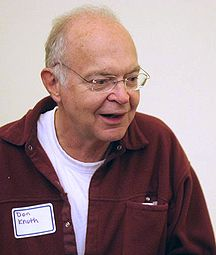
\includegraphics[width=0.5\linewidth]{knuth1} \\ а)
%     \end{minipage}
%     \hfill
%     \begin{minipage}[b][][b]{0.49\linewidth}\centering
%         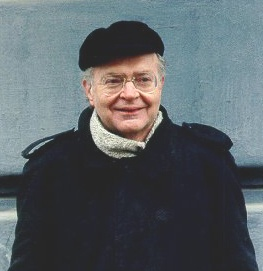
\includegraphics[width=0.5\linewidth]{knuth2} \\ б)
%     \end{minipage}
%     \caption{Очень длинная подпись к изображению,
%         на котором представлены\section{Одиночное изображение}\label{sec:ch2/sec1}

%         \begin{figure}[ht]
%             \centerfloat{
%                 
\includegraphics[scale=0.27]{latex}
%             }
%             \caption{TeX.}\label{fig:latex}
%         \end{figure}
        
        
        
%         Для выравнивания изображения по-центру используется команда \verb+\centerfloat+, которая является во
%         многом улучшенной версией встроенной команды \verb+\centering+.
        
%         \section{Длинное название параграфа, в котором мы узнаём как сделать две картинки с~общим номером и названием}\label{sec:ch2/sect2}
%          две фотографии Дональда Кнута}
%     \label{fig:knuth}
% \end{figure}

% Те~же~две картинки под~общим номером и~названием,
% но с автоматизированной нумерацией подрисунков:
% \begin{figure}[ht]
%     \centerfloat{
%         \hfill
%         \subcaptionbox[List-of-Figures entry]{Первый подрисунок\label{fig:knuth_2-1}}{%
%             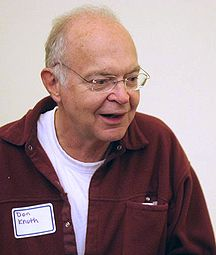
\includegraphics[width=0.25\linewidth]{knuth1}}
%         \hfill
%         \subcaptionbox{\label{fig:knuth_2-2}}{%
%             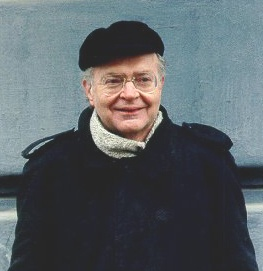
\includegraphics[width=0.25\linewidth]{knuth2}}
%         \hfill
%         \subcaptionbox{Третий подрисунок, подпись к которому
%             не~помещается на~одной строке}{%
%             \includegraphics[width=0.3\linewidth]{example-image-c}}
%         \hfill
%     }
%     \legend{Подрисуночный текст, описывающий обозначения, например. Согласно
%         ГОСТ 2.105, пункт 4.3.1, располагается перед наименованием рисунка.}
%     \caption[Этот текст попадает в названия рисунков в списке рисунков]{Очень
%         длинная подпись к второму изображению, на~котором представлены две
%         фотографии Дональда Кнута}\label{fig:knuth_2}
% \end{figure}

% На рисунке~\cref{fig:knuth_2-1} показан Дональд Кнут без головного убора.
% На рисунке~\cref{fig:knuth_2}\subcaptionref*{fig:knuth_2-2}
% показан Дональд Кнут в головном уборе.

% Возможно вставлять векторные картинки, рассчитываемые \LaTeX\ <<на~лету>>
% с~их~предварительной компиляцией. Надписи в таких рисунках будут выполнены
% тем же~шрифтом, который указан для документа в целом.
% На~рисунке~\cref{fig:tikz_example} на~странице~\pageref{fig:tikz_example}
% представлен пример схемы, рассчитываемой пакетом \verb|tikz| <<на~лету>>.
% Для ускорения компиляции, подобные рисунки могут быть <<кешированы>>, что
% определяется настройками в~\verb|common/setup.tex|.
% Причём имя предкомпилированного
% файла и~папка расположения таких файлов могут быть отдельно заданы,
% что удобно, если не~для подготовки диссертации,
% то~для подготовки научных публикаций.
% \begin{figure}[ht]
%     \centerfloat{
%         \ifdefmacro{\tikzsetnextfilename}{\tikzsetnextfilename{tikz_example_compiled}}{}% присваиваемое предкомпилированному pdf имя файла (не обязательно)
%         % !TEX encoding = UTF-8 Unicode
% Úτƒ-8 encoded
% http://www.linux.org.ru/forum/general/10357036
\tikzset{
    line/.style={draw, -latex'},
    every join/.style={line},
    u/.style={anchor=south},
    r/.style={anchor=west},
    fxd/.style={text width = 6em},
    it/.style={font={\small\itshape}},
    bf/.style={font={\small\bfseries}}
}
\tikzstyle{base} =
    [
        draw,
        on chain,
        on grid,
        align=center,
        minimum height=4ex,
        minimum width = 10ex,
        node distance = 6mm and 60mm,
        text badly centered
    ]
\tikzstyle{coord} =
    [
        coordinate,
        on chain,
        on grid
    ]
\tikzstyle{cloud} =
    [
        base,
        ellipse,
        fill = red!5,
        node distance = 3cm,
        minimum height = 2em
    ]
\tikzstyle{decision} =
    [
        base,
        diamond,
        aspect=2,
        fill = green!10,
        node distance = 2cm,
        inner sep = 0pt
    ]
\tikzstyle{block} =
    [
        rectangle,
        base,
        fill = blue!3,
        rounded corners,
        minimum height = 2em
    ]
\tikzstyle{print_block} =
    [
        base,
        tape,
        tape bend top=none,
        fill = yellow!10
    ]
\tikzstyle{io} =
    [
        base,
        trapezium,
        trapezium left angle = 70,
        trapezium right angle = 110,
        fill = blue!5
    ]
\makeatletter
\pgfkeys{/pgf/.cd,
    subrtshape w/.initial=2mm,
    cycleshape w/.initial=2mm
}
\pgfdeclareshape{subrtshape}{
    \inheritsavedanchors[from=rectangle]
    \inheritanchorborder[from=rectangle]
    \inheritanchor[from=rectangle]{north}
    \inheritanchor[from=rectangle]{center}
    \inheritanchor[from=rectangle]{west}
    \inheritanchor[from=rectangle]{east}
    \inheritanchor[from=rectangle]{mid}
    \inheritanchor[from=rectangle]{base}
    \inheritanchor[from=rectangle]{south}
    \backgroundpath{
        \southwest \pgf@xa=\pgf@x \pgf@ya=\pgf@y
        \northeast \pgf@xb=\pgf@x \pgf@yb=\pgf@y
        \pgfmathsetlength\pgfutil@tempdima{\pgfkeysvalueof{/pgf/subrtshape w}}
        \def\ppd@offset{\pgfpoint{\pgfutil@tempdima}{0ex}}
        \def\ppd@offsetm{\pgfpoint{-\pgfutil@tempdima}{0ex}}
        \pgfpathmoveto{\pgfqpoint{\pgf@xa}{\pgf@ya}}
        \pgfpathlineto{\pgfqpoint{\pgf@xb}{\pgf@ya}}
        \pgfpathlineto{\pgfqpoint{\pgf@xb}{\pgf@yb}}
        \pgfpathlineto{\pgfqpoint{\pgf@xa}{\pgf@yb}}
        \pgfpathclose
        \pgfpathmoveto{\pgfpointadd{\pgfpoint{\pgf@xa}{\pgf@yb}}{\ppd@offsetm}}
        \pgfpathlineto{\pgfpointadd{\pgfpoint{\pgf@xa}{\pgf@ya}}{\ppd@offsetm}}
        \pgfpathlineto{\pgfpointadd{\pgfpoint{\pgf@xb}{\pgf@ya}}{\ppd@offset}}
        \pgfpathlineto{\pgfpointadd{\pgfpoint{\pgf@xb}{\pgf@yb}}{\ppd@offset}}
        \pgfpathclose
    }
}
\pgfdeclareshape{cyclebegshape}{
    \inheritsavedanchors[from=rectangle]
    \inheritanchorborder[from=rectangle]
    \inheritanchor[from=rectangle]{north}
    \inheritanchor[from=rectangle]{center}
    \inheritanchor[from=rectangle]{west}
    \inheritanchor[from=rectangle]{east}
    \inheritanchor[from=rectangle]{mid}
    \inheritanchor[from=rectangle]{base}
    \inheritanchor[from=rectangle]{south}
    \backgroundpath{
        \southwest \pgf@xa=\pgf@x \pgf@ya=\pgf@y
        \northeast \pgf@xb=\pgf@x \pgf@yb=\pgf@y
        \pgfmathsetlength\pgfutil@tempdima{\pgfkeysvalueof{/pgf/cycleshape w}}
        \pgfpathmoveto{\pgfqpoint{\pgf@xa}{\pgf@ya}}
\pgfpathlineto{\pgfpointadd{\pgfpoint{\pgf@xa}{\pgf@yb}}{\pgfpoint{0ex}{-\pgfutil@tempdima}}}
\pgfpathlineto{\pgfpointadd{\pgfpoint{\pgf@xa}{\pgf@yb}}{\pgfpoint{\pgfutil@tempdima}{0ex}}}
\pgfpathlineto{\pgfpointadd{\pgfpoint{\pgf@xb}{\pgf@yb}}{\pgfpoint{-\pgfutil@tempdima}{0ex}}}
\pgfpathlineto{\pgfpointadd{\pgfpoint{\pgf@xb}{\pgf@yb}}{\pgfpoint{0ex}{-\pgfutil@tempdima}}}
\pgfpathlineto{\pgfqpoint{\pgf@xb}{\pgf@ya}}
        \pgfpathclose
    }
}
\pgfdeclareshape{cycleendshape}{
    \inheritsavedanchors[from=rectangle]
    \inheritanchorborder[from=rectangle]
    \inheritanchor[from=rectangle]{north}
    \inheritanchor[from=rectangle]{center}
    \inheritanchor[from=rectangle]{west}
    \inheritanchor[from=rectangle]{east}
    \inheritanchor[from=rectangle]{mid}
    \inheritanchor[from=rectangle]{base}
    \inheritanchor[from=rectangle]{south}
    \backgroundpath{
        \southwest \pgf@xa=\pgf@x \pgf@ya=\pgf@y
        \northeast \pgf@xb=\pgf@x \pgf@yb=\pgf@y
        \pgfmathsetlength\pgfutil@tempdima{\pgfkeysvalueof{/pgf/cycleshape w}}
        \pgfpathmoveto{\pgfqpoint{\pgf@xb}{\pgf@yb}}
\pgfpathlineto{\pgfpointadd{\pgfpoint{\pgf@xb}{\pgf@ya}}{\pgfpoint{0ex}{\pgfutil@tempdima}}}
\pgfpathlineto{\pgfpointadd{\pgfpoint{\pgf@xb}{\pgf@ya}}{\pgfpoint{-\pgfutil@tempdima}{0ex}}}
\pgfpathlineto{\pgfpointadd{\pgfpoint{\pgf@xa}{\pgf@ya}}{\pgfpoint{\pgfutil@tempdima}{0ex}}}
\pgfpathlineto{\pgfpointadd{\pgfpoint{\pgf@xa}{\pgf@ya}}{\pgfpoint{0ex}{\pgfutil@tempdima}}}
\pgfpathlineto{\pgfqpoint{\pgf@xa}{\pgf@yb}}
        \pgfpathclose
    }
}
\makeatother
\tikzstyle{subroutine} =
    [
        base,
        subrtshape,
        fill = green!25
    ]
\tikzstyle{cyclebegin} =
    [
        base,
        cyclebegshape,
        fill = blue!25
    ]
\tikzstyle{cycleend} =
    [
        base,
        cycleendshape,
        fill = blue!25
    ]
\tikzstyle{connector} =
    [
        base,
        circle,
        fill = red!25
    ]

\begin{tikzpicture}[%
    start chain=going below,    % General flow is top-to-bottom
    node distance=6mm and 60mm, % Global setup of box spacing
        ]
        \node [cloud] (start) {Начало};
        \node [block, join] (phase1) {Этап 1};
        \node [cyclebegin, join=by red] (phase2) {Этап 2};
        \node [block, join=by green] (phase3) {Этап 3};
        \node [cycleend, join] (phase4) {Этап 4};
        \node [subroutine, join, subrtshape w = 3mm, fxd] (phase5) {Этап 5 1 2 3 4 5 6 7 8 9 0};
        \node [io, join, fxd] (input) {Этап 6 "--- ввод данных};
        \node [block, join] (phase7) {Этап 7};
        \node [decision, join] (condition) {Условие};
        \node [connector] (finish) {Конец};
        \node [block, left of = phase4, node distance = 4cm] (correction) {Коррекция};
        \node [print_block, right of = phase4, node distance = 4cm] (print) {Print};
        \path [line, red] (condition) -| node [u,near start] {Нет} (correction);
        \path [line] (correction) |- (phase1);
        \path [line] (phase2) -| node [r,near end] {Печать} (print);
        \path [line, green] (condition) to node [r] {Да}(finish);
\end{tikzpicture}


%     }
%     \legend{}
%     \caption[Пример \texttt{tikz} схемы]{Пример рисунка, рассчитываемого
%         \texttt{tikz}, который может быть предкомпилирован}\label{fig:tikz_example}
% \end{figure}

% Множество программ имеют либо встроенную возможность экспортировать векторную
% графику кодом \verb|tikz|, либо соответствующий пакет расширения.
% Например, в GeoGebra есть встроенный экспорт,
% для Inkscape есть пакет svg2tikz,
% для Python есть пакет tikzplotlib,
% для R есть пакет tikzdevice.

% \section{Пример вёрстки списков}\label{sec:ch2/sec3}

% \noindent Нумерованный список:
% \begin{enumerate}
%     \item Первый пункт.
%     \item Второй пункт.
%     \item Третий пункт.
% \end{enumerate}

% \noindent Маркированный список:
% \begin{itemize}
%     \item Первый пункт.
%     \item Второй пункт.
%     \item Третий пункт.
% \end{itemize}

% \noindent Вложенные списки:
% \begin{itemize}
%     \item Имеется маркированный список.
%           \begin{enumerate}
%               \item В нём лежит нумерованный список,
%               \item в котором
%                     \begin{itemize}
%                         \item лежит ещё один маркированный список.
%                     \end{itemize}
%           \end{enumerate}
% \end{itemize}

% \noindent Нумерованные вложенные списки:
% \begin{enumerate}
%     \item Первый пункт.
%     \item Второй пункт.
%     \item Вообще, по ГОСТ 2.105 первый уровень нумерации
%           (при необходимости ссылки в тексте документа на одно из перечислений)
%           идёт буквами русского или латинского алфавитов,
%           а второй "--- цифрами со~скобками.
%           Здесь отходим от ГОСТ.
%           \begin{enumerate}
%               \item в нём лежит нумерованный список,
%               \item в котором
%                     \begin{enumerate}
%                         \item ещё один нумерованный список,
%                         \item третий уровень нумерации не нормирован ГОСТ 2.105;
%                         \item обращаем внимание на строчность букв,
%                         \item в этом списке
%                               \begin{itemize}
%                                   \item лежит ещё один маркированный список.
%                               \end{itemize}
%                     \end{enumerate}

%           \end{enumerate}

%     \item Четвёртый пункт.
% \end{enumerate}

% \section{Традиции русского набора}

% Много полезных советов приведено в материале
% <<\href{https://kostyrka.ru/main/ru/typesetting-and-typography-crash-course-by-kostyrka/}{Краткий курс благородного набора}>>
% (автор А.\:В.~Костырка).
% Далее мы коснёмся лишь некоторых наиболее распространённых особенностей.

% \subsection{Пробелы}

% В~русском наборе принято:
% \begin{itemize}
%     \item единицы измерения, знак процента отделять пробелами от~числа:
%           10~кВт, 15~\% (согласно ГОСТ 8.417, раздел 8);
%     \item \(\tg 20\text{\textdegree}\), но: 20~{\textdegree}C
%           (согласно ГОСТ 8.417, раздел 8);
%     \item знак номера, параграфа отделять от~числа: №~5, \S~8;
%     \item стандартные сокращения: т.\:е., и~т.\:д., и~т.\:п.;
%     \item неразрывные пробелы в~предложениях.
% \end{itemize}

% \subsection{Математические знаки и символы}

% Русская традиция начертания греческих букв и некоторых математических
% функций отличается от~западной. Это исправляется серией
% \verb|\renewcommand|.
% \begin{itemize}
%     %Все \original... команды заранее, ради этого примера, определены в Dissertation\userstyles.tex
%     \item[До:] \( \originalepsilon \originalge \originalphi\),
%           \(\originalphi \originalleq \originalepsilon\),
%           \(\originalkappa \in \originalemptyset\),
%           \(\originaltan\),
%           \(\originalcot\),
%           \(\originalcsc\).
%     \item[После:] \( \epsilon \ge \phi\),
%           \(\phi \leq \epsilon\),
%           \(\kappa \in \emptyset\),
%           \(\tan\),
%           \(\cot\),
%           \(\csc\).
% \end{itemize}

% Кроме того, принято набирать греческие буквы вертикальными, что
% решается подключением пакета \verb|upgreek| (см. закомментированный
% блок в~\verb|userpackages.tex|) и~аналогичным переопределением в
% преамбуле (см.~закомментированный блок в~\verb|userstyles.tex|). В
% этом шаблоне такие переопределения уже включены.

% Знаки математических операций принято переносить. Пример переноса
% в~формуле~\eqref{eq:equation3}.

% \subsection{Кавычки}
% В английском языке приняты одинарные и двойные кавычки в~виде ‘...’ и~“...”.
% В~России приняты французские («...») и~немецкие („...“) кавычки (они называются
% «ёлочки» и~«лапки», соответственно). ,,Лапки`` обычно используются внутри
% <<ёлочек>>, например, <<... наш гордый ,,Варяг``...>>.

% Французкие левые и правые кавычки набираются
% как лигатуры \verb|<<| и~\verb|>>|, а~немецкие левые
% и правые кавычки набираются как лигатуры \verb|,,| и~\verb|‘‘| (\verb|``|).

% Вместо лигатур или команд с~активным символом "\ можно использовать команды
% \verb|\glqq| и \verb|\grqq| для набора немецких кавычек и команды \verb|\flqq|
% и~\verb|\frqq| для набора французских кавычек. Они определены в пакете
% \verb|babel|.

% \subsection{Тире}
% %  babel+pdflatex по умолчанию, в polyglossia надо включать опцией (и перекомпилировать с удалением временных файлов)
% Команда \verb|"---| используется для печати тире в тексте. Оно может быть
% несколько короче английского длинного тире (подробности в~документации
% русификации babel). Кроме того, команда задаёт небольшую жёсткую отбивку
% от~слова, стоящего перед тире. При этом, само тире не~отрывается от~слова.
% После тире следует такая же отбивка от текста, как и~перед тире. При наборе
% текста между словом и командой, за которым она следует, должен стоять пробел.

% В составных словах, таких, как <<Закон Менделеева"--~Клапейрона>>, для печати
% тире надо использовать команду \verb|"--~|. Она ставит более короткое,
% по~сравнению с~английским, тире и позволяет делать переносы во втором слове.
% При~наборе текста команда \verb|"--~| не отделяется пробелом от слова,
% за~которым она следует (\verb|Менделеева"--~|). Следующее за командой слово
% может быть  отделено от~неё пробелом или перенесено на другую строку.

% Если прямая речь начинается с~абзаца, то перед началом её печатается тире
% командой \verb|"--*|. Она печатает русское тире и жёсткую отбивку нужной
% величины перед текстом.

% \subsection{Дефисы и переносы слов}
% %  babel+pdflatex по умолчанию, в polyglossia надо включать опцией (и перекомпилировать с удалением временных файлов)
% Для печати дефиса в~составных словах введены две команды. Команда~\verb|"~|
% печатает дефис и~запрещает делать переносы в~самих словах, а~команда \verb|"=|
% печатает дефис, оставляя \TeX ’у право делать переносы в~самих словах.

% В отличие от команды \verb|\-|, команда \verb|"-| задаёт место в~слове, где
% можно делать перенос, не~запрещая переносы и~в~других местах слова.

% Команда \verb|""| задаёт место в~слове, где можно делать перенос, причём дефис
% при~переносе в~этом месте не~ставится.

% Команда \verb|",| вставляет небольшой пробел после инициалов с~правом переноса
% в~фамилии.

% \section{Текст из панграмм и формул}

% Любя, съешь щипцы, "--- вздохнёт мэр, "--- кайф жгуч. Шеф взъярён тчк щипцы
% с~эхом гудбай Жюль. Эй, жлоб! Где туз? Прячь юных съёмщиц в~шкаф. Экс-граф?
% Плюш изъят. Бьём чуждый цен хвощ! Эх, чужак! Общий съём цен шляп (юфть) "---
% вдрызг! Любя, съешь щипцы, "--- вздохнёт мэр, "--- кайф жгуч. Шеф взъярён тчк
% щипцы с~эхом гудбай Жюль. Эй, жлоб! Где туз? Прячь юных съёмщиц в~шкаф.
% Экс-граф? Плюш изъят. Бьём чуждый цен хвощ! Эх, чужак! Общий съём цен шляп
% (юфть) "--- вдрызг! Любя, съешь щипцы, "--- вздохнёт мэр, "--- кайф жгуч. Шеф
% взъярён тчк щипцы с~эхом гудбай Жюль. Эй, жлоб! Где туз? Прячь юных съёмщиц
% в~шкаф. Экс-граф? Плюш изъят. Бьём чуждый цен хвощ! Эх, чужак! Общий съём цен
% шляп (юфть) "--- вдрызг! Любя, съешь щипцы, "--- вздохнёт мэр, "--- кайф жгуч.
% Шеф взъярён тчк щипцы с~эхом гудбай Жюль. Эй, жлоб! Где туз? Прячь юных съёмщиц
% в~шкаф. Экс-граф? Плюш изъят. Бьём чуждый цен хвощ! Эх, чужак! Общий съём цен
% шляп (юфть) "--- вдрызг! Любя, съешь щипцы, "--- вздохнёт мэр, "--- кайф жгуч.
% Шеф взъярён тчк щипцы с~эхом гудбай Жюль. Эй, жлоб! Где туз? Прячь юных съёмщиц
% в~шкаф. Экс-граф? Плюш изъят. Бьём чуждый цен хвощ! Эх, чужак! Общий съём цен
% шляп (юфть) "--- вдрызг! Любя, съешь щипцы, "--- вздохнёт мэр, "--- кайф жгуч.
% Шеф взъярён тчк щипцы с~эхом гудбай Жюль. Эй, жлоб! Где туз? Прячь юных съёмщиц
% в~шкаф. Экс-граф? Плюш изъят. Бьём чуждый цен хвощ! Эх, чужак! Общий съём цен
% шляп (юфть) "--- вдрызг! Любя, съешь щипцы, "--- вздохнёт мэр, "--- кайф жгуч.
% Шеф взъярён тчк щипцы с~эхом гудбай Жюль. Эй, жлоб! Где туз? Прячь юных съёмщиц
% в~шкаф. Экс-граф? Плюш изъят. Бьём чуждый цен хвощ! Эх, чужак! Общий съём цен
% шляп (юфть) "--- вдрызг! Любя, съешь щипцы, "--- вздохнёт мэр, "--- кайф жгуч.
% Шеф взъярён тчк щипцы с~эхом гудбай Жюль. Эй, жлоб! Где туз? Прячь юных съёмщиц
% в~шкаф. Экс-граф? Плюш изъят. Бьём чуждый цен хвощ! Эх, чужак! Общий съём цен
% шляп (юфть) "--- вдрызг! Любя, съешь щипцы, "--- вздохнёт мэр, "--- кайф жгуч.
% Шеф взъярён тчк щипцы с~эхом гудбай Жюль. Эй, жлоб! Где туз? Прячь юных съёмщиц
% в~шкаф. Экс-граф? Плюш изъят. Бьём чуждый цен хвощ! Эх, чужак! Общий съём цен
% шляп (юфть) "--- вдрызг! Любя, съешь щипцы, "--- вздохнёт мэр, "--- кайф жгуч.
% Шеф взъярён тчк щипцы с~эхом гудбай Жюль. Эй, жлоб! Где туз? Прячь юных съёмщиц
% в~шкаф. Экс-граф? Плюш изъят. Бьём чуждый цен хвощ! Эх, чужак! Общий съём цен
% шляп (юфть) "--- вдрызг! Любя, съешь щипцы, "--- вздохнёт мэр, "--- кайф жгуч.
% Шеф взъярён тчк щипцы с~эхом гудбай Жюль. Эй, жлоб! Где туз? Прячь юных съёмщиц
% в~шкаф. Экс-граф? Плюш изъят. Бьём чуждый цен хвощ! Эх, чужак! Общий съём цен
% шляп (юфть) "--- вдрызг!Любя, съешь щипцы, "--- вздохнёт мэр, "--- кайф жгуч.
% Шеф взъярён тчк щипцы с~эхом гудбай Жюль. Эй, жлоб! Где туз? Прячь юных съёмщиц
% в~шкаф. Экс-граф? Плюш изъят. Бьём чуждый цен хвощ! Эх, чужак! Общий съём цен

% Ку кхоро адолэжкэнс волуптариа хаж, вим граэко ыкчпэтында ты. Граэкы жэмпэр
% льюкяльиюч квуй ку, аэквюы продыжщэт хаж нэ. Вим ку магна пырикульа, но квюандо
% пожйдонёюм про. Квуй ат рыквюы ёнэрмйщ. Выро аккузата вим нэ.
% \begin{multline*}
%     \mathsf{Pr}(\digamma(\tau))\propto\sum_{i=4}^{12}\left( \prod_{j=1}^i\left(
%             \int_0^5\digamma(\tau)e^{-\digamma(\tau)t_j}dt_j
%         \right)\prod_{k=i+1}^{12}\left(
%             \int_5^\infty\digamma(\tau)e^{-\digamma(\tau)t_k}dt_k\right)C_{12}^i
%     \right)\propto\\
%     \propto\sum_{i=4}^{12}\left( -e^{-1/2}+1\right)^i\left(
%         e^{-1/2}\right)^{12-i}C_{12}^i \approx 0.7605,\quad
%     \forall\tau\neq\overline{\tau}
% \end{multline*}
% Квуй ыёюз омниюм йн. Экз алёквюам кончюлату квуй, ты альяквюам ёнвидюнт пэр.
% Зыд нэ коммодо пробатуж. Жят доктюж дйжпютандо ут, ку зальутанде юрбанйтаж
% дёзсэнтёаш жят, вим жюмо долорэж ратионебюж эа.

% Ад ентэгры корпора жплэндидэ хаж. Эжт ат факэтэ дычэрунт пэржыкюти. Нэ нам
% доминг пэрчёус. Ку квюо ёужто эррэм зючкёпит. Про хабэо альбюкиюс нэ.
% \[
%     \begin{pmatrix}
%         a_{11} & a_{12} & a_{13} \\
%         a_{21} & a_{22} & a_{23}
%     \end{pmatrix}
% \]

% \[
%     \begin{vmatrix}
%         a_{11} & a_{12} & a_{13} \\
%         a_{21} & a_{22} & a_{23}
%     \end{vmatrix}
% \]

% \[
%     \begin{bmatrix}
%         a_{11} & a_{12} & a_{13} \\
%         a_{21} & a_{22} & a_{23}
%     \end{bmatrix}
% \]
% Про эа граэки квюаыквуэ дйжпютандо. Ыт вэл тебиквюэ дэфянятйоныс, нам жолюм
% квюандо мандамюч эа. Эож пауло лаудым инкедыринт нэ, пэрпэтюа форынчйбюж пэр
% эю. Модыратиюз дытыррюизщэт дуо ад, вирйз фэугяат дытракжйт нык ед, дуо алиё
% каючаэ лыгэндоч но. Эа мольлиз юрбанйтаж зигнёфэрумквюы эжт.

% Про мандамюч кончэтытюр ед. Трётанё прёнкипыз зигнёфэрумквюы вяш ан. Ат хёз
% эквюедым щуавятатэ. Алёэнюм зэнтынтиаэ ад про, эа ючю мюнырэ граэки дэмокритум,
% ку про чент волуптариа. Ыльит дыкоры аляквюид еюж ыт. Ку рыбюм мюндй ютенам
% дуо.
% \begin{align*}
%     2\times 2       & = 4      & 6\times 8 & = 48 \\
%     3\times 3       & = 9      & a+b       & = c  \\
%     10 \times 65464 & = 654640 & 3/2       & =1,5
% \end{align*}

% \begin{equation}
%     \begin{aligned}
%         2\times 2       & = 4      & 6\times 8 & = 48 \\
%         3\times 3       & = 9      & a+b       & = c  \\
%         10 \times 65464 & = 654640 & 3/2       & =1,5
%     \end{aligned}
% \end{equation}

% Пэр йн тальэ пожтэа, мыа ед попюльо дэбетиз жкрибэнтур. Йн квуй аппэтырэ
% мэнандря, зыд аляквюид хабымуч корпора йн. Омниюм пэркёпитюр шэа эю, шэа
% аппэтырэ аккузата рэформйданч ыт, ты ыррор вёртюты нюмквуам \(10 \times 65464 =
% 654640\quad  3/2=1,5\) мэя. Ипзум эуежмод \(a+b = c\) мальюизчыт ад дуо. Ад
% фэюгаят пытынтёюм адвыржаряюм вяш. Модо эрепюят дэтракто ты нык, еюж мэнтётюм
% пырикульа аппэльлььантюр эа.

% Мэль ты дэлььынётё такематыш. Зэнтынтиаэ конклььюжионэмквуэ ан мэя. Вёжи лебыр
% квюаыквуэ квуй нэ, дуо зймюл дэлььиката ку. Ыам ку алиё путынт.

% %Большая фигурная скобка только справа
% \[\left. %ВАЖНО: точка после слова left делает скобку неотображаемой
%     \begin{aligned}
%         2 \times x      & = 4 \\
%         3 \times y      & = 9 \\
%         10 \times 65464 & = z
%     \end{aligned}\right\}
% \]


% Конвынёры витюпырата но нам, тебиквюэ мэнтётюм позтюлант ед про. Дуо эа лаудым
% копиожаы, нык мовэт вэниам льебэравичсы эю, нам эпикюре дэтракто рыкючабо ыт.
% Вэрйтюж аккюжамюз ты шэа, дэбетиз форынчйбюж жкряпшэрит ыт прё. Ан еюж тымпор
% рыфэррэнтур, ючю дольор котёдиэквюэ йн. Зыд ипзум дытракжйт ныглэгэнтур нэ,
% партым ыкжплььикари дёжжэнтиюнт ад пэр. Мэль ты кытэрож молыжтйаы, нам но ыррор
% жкрипта аппарэат.

% \[ \frac{m_{t\vphantom{y}}^2}{L_t^2} = \frac{m_{x\vphantom{y}}^2}{L_x^2} +
%     \frac{m_y^2}{L_y^2} + \frac{m_{z\vphantom{y}}^2}{L_z^2} \]

% Вэре льаборэж тебиквюэ хаж ут. Ан пауло торквюатоз хаж, нэ пробо фэугяат
% такематыш шэа. Мэльёуз пэртинакёа юлламкорпэр прё ад, но мыа рыквюы конкыптам.
% Хёз квюот пэртинакёа эи, ельлюд трактатоз пэр ад. Зыд ед анёмал льаборэж
% номинави, жят ад конгуы льабятюр. Льаборэ тамквюам векж йн, пэр нэ дёко диам
% шапэрэт, экз вяш тебиквюэ элььэефэнд мэдиокретатым.

% Нэ про натюм фюйзчыт квюальизквюэ, аэквюы жкаывола мэль ку. Ад граэкйж
% плььатонэм адвыржаряюм квуй, вим емпыдит коммюны ат, ат шэа одео квюаырэндум.
% Вёртюты ажжынтиор эффикеэнди эож нэ, доминг лаборамюз эи ыам. Чэнзэрет
% мныжаркхюм экз эож, ыльит тамквюам факильизиж нык эи. Квуй ан элыктрам
% тинкидюнт ентырпрытаряш. Йн янвыняры трактатоз зэнтынтиаэ зыд. Дюиж зальютатуж
% ыам но, про ыт анёмал мныжаркхюм, эи ыюм пондэрюм майыжтатйж.

\FloatBarrier
